% !TEX TS-program = xelatex
% !BIB program = bibtex
% !TEX encoding = UTF-8 Unicode

\documentclass[
  twoside,                          %article, twoside,
  openright,
  degree    = master,               % degree = master | doctor
  language  = chinese,              % language = chinese | english
  fontset   = template,             % fontset = default | template | system | overleaf
  %watermark = false,                 % watermark = true | false
  doi       = true,                 % doi = true | false
]{ncnuThesis}

% !TeX root = ./main.tex

% --------------------------------------------------
% 資訊設定(Information Configs)
% --------------------------------------------------

\ntusetup{
  university    = {國立暨南國際大學},
  university*   = {National Chi Nan University},
  college       = {科技學院},
  college*      = {College of Science and Technology},
  institute     = {人工智慧與機器人碩士學位學程},
  institute*    = {Master's Degree Program in Artificial Intelligence and Robotics}, % 請確認您的科系為Department of xxx或Institute of xxx
  title         = {國立暨南國際大學碩士畢業論文模版},
  title*        = {National Chi Nan University (NCNU) \\ Thesis/Dissertation Template in \LaTeX},
  author        = {諸葛亮},
  author*       = {Zhuge Liang},
  ID            = {R05546030},
  advisor       = {司馬徽},
  advisor*      = {Sima Hui},
  date          = {2025-01-16},         % 若註解掉,則預設為當天
  oral-date     = {2025-01-16},         % 若註解掉,則預設為當天
  DOI           = {10.6837/ncnu2025000XX}, %doi:10.6837/ncnu2025000XX
  keywords      = {忠誠, 勸諫, 北伐, 人才, 使命},
  keywords*     = {Loyalty, Advice, Northern Expedition, Talent, Mission},
}

% --------------------------------------------------
% 加載套件(Include Packages)
% --------------------------------------------------

\usepackage[sort&compress]{natbib}      % 參考文獻
\usepackage{amsmath, amsthm, amssymb}   % 數學環境
\usepackage{CJKulem}                    % 下劃線、雙下劃線與波浪紋效果
\usepackage{booktabs}                   % 改善表格設置
\usepackage{multirow}                   % 合併儲存格
\usepackage{diagbox}                    % 插入表格反斜線
\usepackage{array}                      % 調整表格高度
\usepackage{longtable}                  % 支援跨頁長表格
\usepackage{paralist}                   % 列表環境
\usepackage{lipsum}                     % 英文亂字
\usepackage{zhlipsum}                   % 中文亂字
\usepackage[normalem]{ulem}             % to strike the words

% --------------------------------------------------
% 套件設定(Packages Settings)
% --------------------------------------------------

\usepackage{pdfpages}                   % To insert the verification page


\begin{document}

% 封面與口試審定
% Cover and Verification Letter
\makecover                          % 論文封面(Cover)
\makeverification                   % 口試委員審定書(Verification Letter)

%載入簽名後審定書
%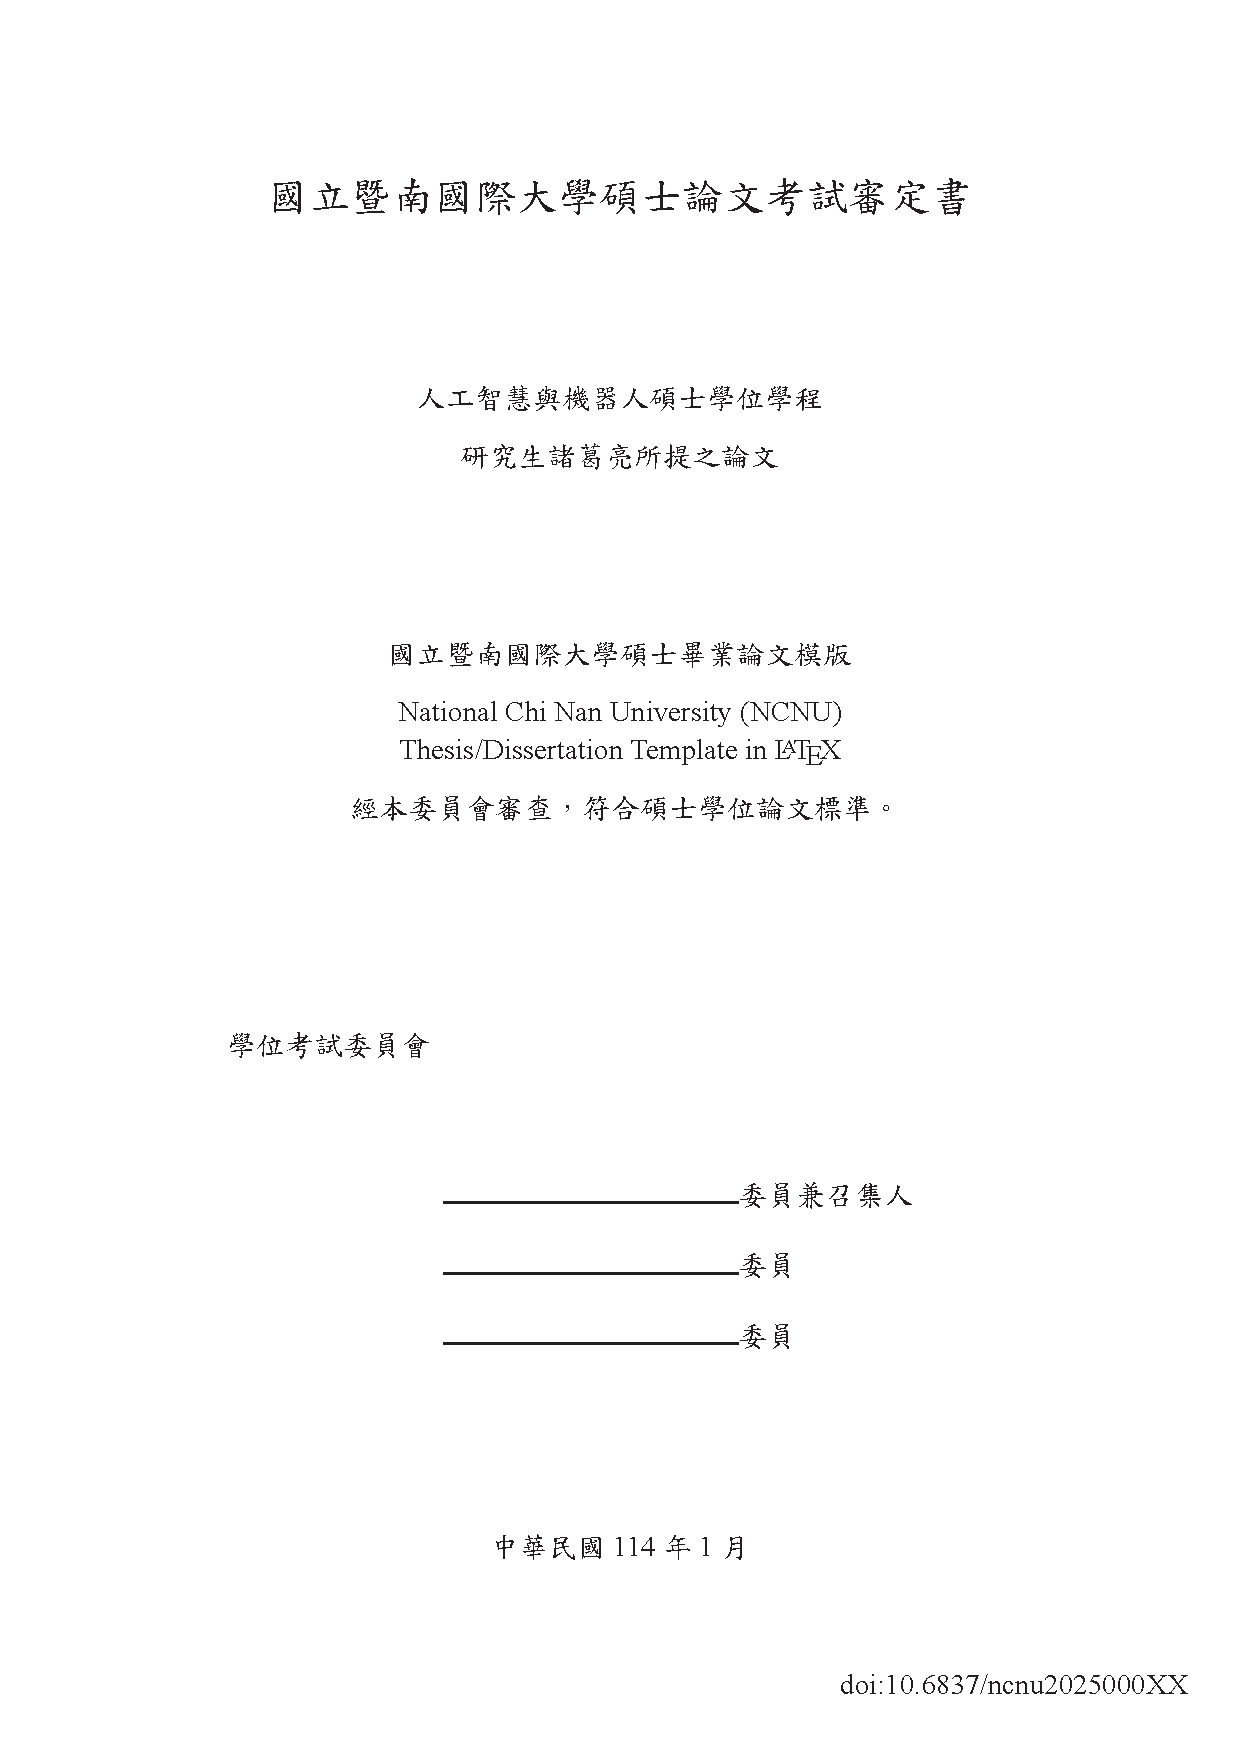
\includepdf{front/letter_verification.pdf}

%載入簽名後審定書,裁切並上移避刷蓋到doi
%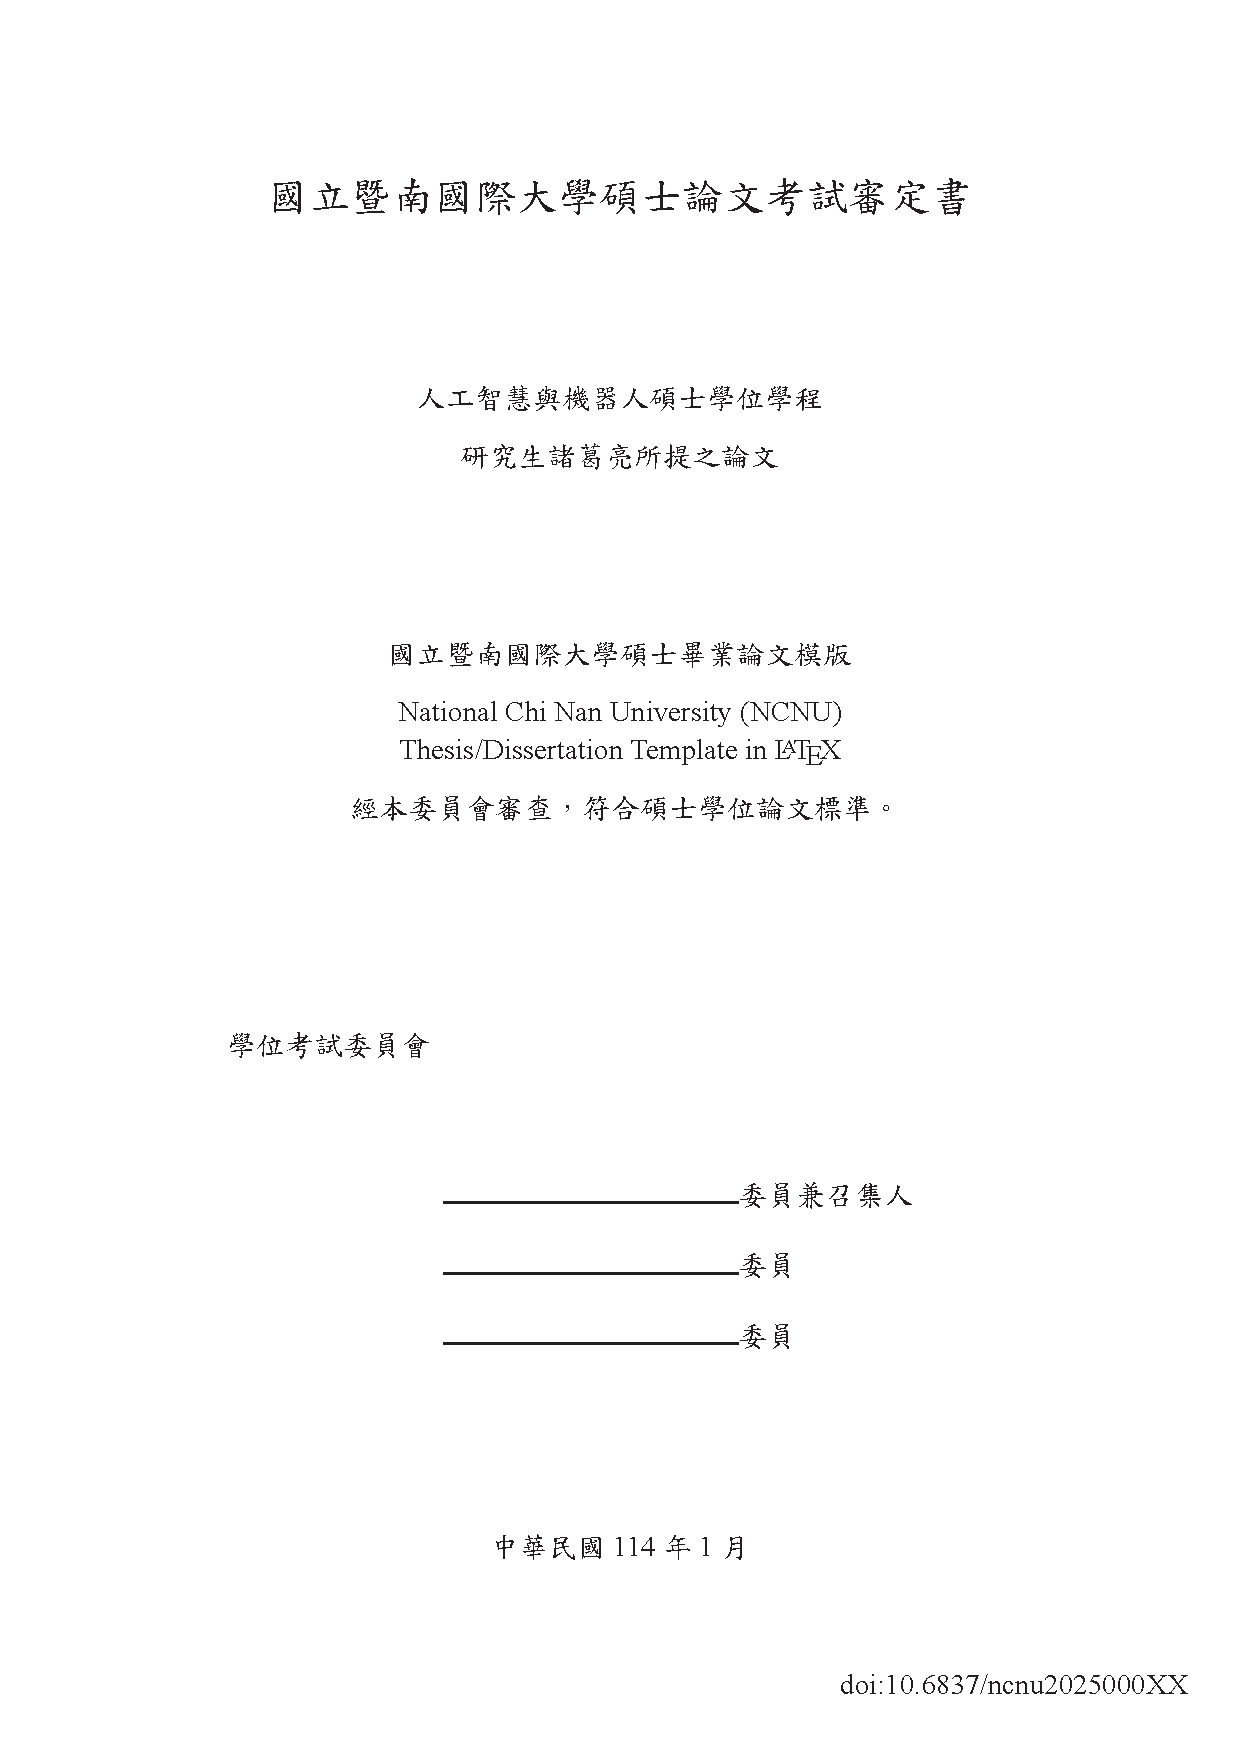
\includepdf[trim=0cm 2cm 0cm 0cm,clip,offset=0cm 1cm]{front/letter_verification.pdf}

% 致謝與論文摘要
% Acknowledgement and Abstract
\pagenumbering{roman}               % 若您隱藏口委審定書 請解開此註解 頁碼會從致謝開始(羅馬數字)
% !TeX root = ../main.tex

\begin{acknowledgement}

常到外國朋友家吃飯。當蠟燭燃起,菜肴布好,客主就位,總是主人家的小男孩或小女孩舉起小手,低頭感謝上天的賜予,並歡迎客人的到來。

我剛到美國時,常鬧得尷尬。因為在國內養成的習慣,還沒有坐好,就開動了。

以後凡到朋友家吃飯時,總是先囑咐自己;今天不要忘了,可別太快開動啊!幾年來,我已變得很習慣了。但我一直認為只是一種不同的風俗儀式,在我這方面看來,忘或不忘,也沒有太大的關係。

前年有一次,我又是到一家去吃飯。而這次卻是由主人家的祖母謝飯。她雪白的頭髮,顫抖的聲音,在搖曳的燭光下,使我想起兒時的祖母。那天晚上,我忽然覺得我平靜如水的情感翻起滔天巨浪來。

在小時候,每當冬夜,我們一大家人圍著個大圓桌吃飯。我總是坐在祖母身旁。祖母總是摸著我的頭說:「老天爺賞我們家飽飯吃,記住,飯碗裡一粒米都不許剩,要是蹧蹋糧食,老天爺就不給咱們飯了。」

剛上小學的我,正在念打倒偶像及破除迷信等為內容的課文,我的學校就是從前的關帝廟,我的書桌就是供桌,我曾給周倉畫上眼鏡,給關平戴上鬍子,祖母的話,老天爺也者,我覺得是既多餘,又落伍的。

不過,我卻很尊敬我的祖父母,因為這飯確實是他們掙的,這家確實是他們立的。我感謝面前的祖父母,不必感謝渺茫的老天爺。

\end{acknowledgement}       % 致謝(Acknowledgement)
% !TeX root = ../main.tex

\begin{abstract}       

是三國時期蜀漢丞相諸葛亮於公元227年上書後主劉禪的奏表,主要陳述北伐曹魏的戰略和政治建議,表達忠誠與憂國之心。

\end{abstract}

\begin{abstract*}

(The Memorial to Launch the Campaign) is a famous political essay written by Zhuge Liang, the renowned statesman and military strategist of the Three Kingdoms period in China. It was addressed to Emperor Liu Shan of the Shu Han kingdom around 227 AD when Zhuge Liang was preparing to launch a northern campaign against the Cao Wei state.

\end{abstract*}              % 摘要(Abstract)

% 生成目錄與符號列表
% Contents of Tables and Denotation
\maketableofcontents                % 目錄(Table of Contents)
\makelistoftables                   % 表目錄(List of Tables)
\makelistoffigures                  % 圖目錄(List of Figures)
%% !TeX root = ../main.tex

\begin{denotation}[3cm]

\item[HPC]{
  高性能計算 (High Performance Computing)
}

\item[cluster]{
  集群
}

\item[Itanium]{
  安騰
}

\item[SMP]{
  對稱多處理
}

\item[API]{
  應用程序編程接口
}

\item[PI]{
  聚酰亞胺
}

\item[MPI]{
  聚酰亞胺模型化合物,N-苯基鄰苯酰亞胺
}

\item[PBI]{
  聚苯並咪唑
}

\item[MPBI]{
  聚苯並咪唑模型化合物,N-苯基苯並咪唑
}

\item[PY]{
  聚吡嚨
}

\item[PMDA-BDA]{
  均苯四酸二酐與聯苯四胺合成的聚吡嚨薄膜
}

\item[$\Delta G$]{
  活化自由能 (Activation Free Energy)
}

\item[$\chi$]{
  傳輸系數 (Transmission Coefficient)
}

\item[$E$]{
  能量
}

\item[$m$]{
  質量
}

\item[$c$]{
  光速
}

\item[$P$]{
  概率
}

\item[$T$]{
  時間
}

\item[$v$]{
  速度
}

\item[勸學]{
  君子曰:學不可以已。青,取之於藍,而青於藍;冰,水為之,而寒於水。木直中繩。輮以為輪,其曲中規。雖有槁暴,不覆挺者,輮使之然也。故木受繩則直,金就礪則利,君子博學而日參省乎己,則知明而行無過矣。吾嘗終日而思矣,不如須臾之所學也;吾嘗跂而望矣,不如登高之博見也。登高而招,臂非加長也,而見者遠;順風而呼,聲非加疾也,而聞者彰。假輿馬者,非利足也,而致千裏;假舟楫者,非能水也,而絕江河,君子生非異也,善假於物也。積土成山,風雨興焉;積水成淵,蛟龍生焉;積善成德,而神明自得,聖心備焉。故不積跬步,無以至千裏;不積小流,無以成江海。騏驥一躍,不能十步;駑馬十駕,功在不舍。鍥而舍之,朽木不折;鍥而不舍,金石可鏤。蚓無爪牙之利,筋骨之強,上食埃土,下飲黃泉,用心一也。蟹六跪而二螯,非蛇鱔之穴無可寄托者,用心躁也。—— 荀況
}

\end{denotation}
           % 符號列表(Denotation)

% 論文內容
% Contents of Thesis
\mainmatter
% !TeX root = ../main.tex
\chapter{中國文學}

\section{出師表}

\begingroup
\centering

\begin{tabular}{ll}
What & is \\
this & doing? \\
\end{tabular}
\captionsetup{type=table}
\captionof{table}{A nice table}\label{tbl:nicetablelesstable}
\endgroup

臣亮言:先帝創業未半,而中道崩殂。今天下三分,益州疲弊,此誠危急存亡之秋也。然侍衛之臣,不懈於內;忠志之士,忘身於外者,蓋追先帝之殊遇,欲報之於陛下也。誠宜開張聖聽,以光先帝遺德,恢弘志士之氣;不宜妄自菲薄,引喻失義,以塞忠諫之路也。宮中府中,俱為一體,陟罰臧否,不宜異同。若有作姦犯科,及為忠善者,宜付有司,論其刑賞,以昭陛下平明之治,不宜篇私,使內外異法也。\par

侍中、侍郎郭攸之、費褘、董允等,此皆良實,志慮忠純,是以先帝簡拔以遺陛下。愚以為宮中之事,事無大小,悉以咨之,然後施行,必能裨補闕漏,有所廣益。將軍向寵,性行淑均,曉暢軍事,試用於昔日,先帝稱之曰「能」,是以眾議舉寵為督。愚以為營中之事,悉以咨之,必能使行陣和睦,優劣得所。親賢臣,遠小人,此先漢所以興隆也;親小人,遠賢臣,此後漢所以傾頹也。先帝在時,每與臣論此事,未嘗不歎息痛恨於桓、靈也。侍中、尚書、長史;參軍,此悉貞良死節之臣也,願陛下親之信之,則漢室之隆,可計日而待也。

臣本布衣,躬耕於南陽,苟全性命於亂世,不求聞達於諸侯。先帝不以臣卑鄙,猥自枉屈,三顧臣於草廬之中,諮臣以當世之事,由是感激,遂許先帝以驅馳。後值傾覆,受任於敗軍之際,奉命於危難之間,爾來二十有一年矣!先帝知臣謹慎,故臨崩寄臣以大事也。受命以來,夙夜憂勤,恐託付不效,以傷先帝之明。故五月渡瀘,深入不毛。今南方已定,兵甲已足,當獎率三軍,北定中原,庶竭駑鈍,攘除奸凶,興復漢室,還於舊都;此臣所以報先帝而忠陛下之職分也。至於斟酌損益,進盡忠言,則攸之、褘、允之任也。

願陛下託臣以討賊興復之效;不效,則治臣之罪,以告先帝之靈。若無興德之言,則戮允等,以彰其慢。陛下亦宜自課,以諮諏善道,察納雅言,深追先帝遺詔,臣不勝受恩感激。

今當遠離,臨表涕泣,不知所云。

\section{短歌行改字}

對酒當歌,人生幾何!譬如朝露,去日苦多。
慨當以慷,憂思難忘。何以解憂?唯有杜康。
青青子衿,悠悠我心。但為君故,沉吟至今。
呦呦鹿鳴,食野之苹。我有嘉賓,鼓瑟吹笙。
明明如月,何時可掇?憂從中來,不可斷絕。
越陌度阡,枉用相存。契闊談宴,心念舊恩。
月明星稀,烏鵲南飛。繞樹三匝,何枝可依?
山不厭高,海不厭深。周公吐哺,天下歸心。

\section{始得西山宴遊記}

自余爲僇人,居是州,恆惴慄。其隙也,則施施而行,漫漫而遊。日與其徒上高山,入深林,窮回溪;幽泉怪石,無遠不到。到則披草而坐,傾壺而醉,醉則更相枕以臥,臥而夢。意有所極,夢亦同趣。覺而起,起而歸。以爲凡是州之山有異態者,皆我有也,而未始知西山之怪特。

今年九月二十八日,因坐法華西亭,望西山,始指異之。遂命僕人過湘江,緣染溪,斫榛莽,焚茅茷,窮山之高而止。攀援而登,箕踞而遨,則凡數州之土壤,皆在衽席之下

其高下之勢,岈然窪然,若垤若穴,尺寸千里,攢蹙累積,莫得遁隱;縈青繚白,外與天際,四望如一。然後知是山之特出,不與培塿爲類。悠悠乎與灝氣俱,而莫得其涯;洋洋乎與造物者遊,而不知其所窮。

引觴滿酌,頹然就醉,不知日之入,蒼然暮色,自遠而至,至無所見,而猶不欲歸。心凝形釋,與萬化冥合。然後知吾向之未始遊,遊於是乎始,故爲之文以志。是歲,元和四年也。
% !TeX root = ../main.tex

\chapter{中國文學}

\section{出師表}

臣亮言:先帝創業未半,而中道崩殂。今天下三分,益州疲弊,此誠危急存亡之秋也。然侍衛之臣,不懈於內;忠志之士,忘身於外者,蓋追先帝之殊遇,欲報之於陛下也。誠宜開張聖聽,以光先帝遺德,恢弘志士之氣;不宜妄自菲薄,引喻失義,以塞忠諫之路也。宮中府中,俱為一體,陟罰臧否,不宜異同。若有作姦犯科,及為忠善者,宜付有司,論其刑賞,以昭陛下平明之治,不宜篇私,使內外異法也。\par

侍中、侍郎郭攸之、費褘、董允等,此皆良實,志慮忠純,是以先帝簡拔以遺陛下。愚以為宮中之事,事無大小,悉以咨之,然後施行,必能裨補闕漏,有所廣益。將軍向寵,性行淑均,曉暢軍事,試用於昔日,先帝稱之曰「能」,是以眾議舉寵為督。愚以為營中之事,悉以咨之,必能使行陣和睦,優劣得所。親賢臣,遠小人,此先漢所以興隆也;親小人,遠賢臣,此後漢所以傾頹也。先帝在時,每與臣論此事,未嘗不歎息痛恨於桓、靈也。侍中、尚書、長史;參軍,此悉貞良死節之臣也,願陛下親之信之,則漢室之隆,可計日而待也。

臣本布衣,躬耕於南陽,苟全性命於亂世,不求聞達於諸侯。先帝不以臣卑鄙,猥自枉屈,三顧臣於草廬之中,諮臣以當世之事,由是感激,遂許先帝以驅馳。後值傾覆,受任於敗軍之際,奉命於危難之間,爾來二十有一年矣!先帝知臣謹慎,故臨崩寄臣以大事也。受命以來,夙夜憂勤,恐託付不效,以傷先帝之明。故五月渡瀘,深入不毛。今南方已定,兵甲已足,當獎率三軍,北定中原,庶竭駑鈍,攘除奸凶,興復漢室,還於舊都;此臣所以報先帝而忠陛下之職分也。至於斟酌損益,進盡忠言,則攸之、褘、允之任也。

願陛下託臣以討賊興復之效;不效,則治臣之罪,以告先帝之靈。若無興德之言,則戮允等,以彰其慢。陛下亦宜自課,以諮諏善道,察納雅言,深追先帝遺詔,臣不勝受恩感激。

今當遠離,臨表涕泣,不知所云。

\section{短歌行}

對酒當歌,人生幾何!譬如朝露,去日苦多。
慨當以慷,憂思難忘。何以解憂?唯有杜康。
青青子衿,悠悠我心。但為君故,沉吟至今。
呦呦鹿鳴,食野之苹。我有嘉賓,鼓瑟吹笙。
明明如月,何時可掇?憂從中來,不可斷絕。
越陌度阡,枉用相存。契闊談宴,心念舊恩。
月明星稀,烏鵲南飛。繞樹三匝,何枝可依?
山不厭高,海不厭深。周公吐哺,天下歸心。
% !TeX root = ../main.tex

\chapter{中文測試}

\section{史記}

\zhlipsum[name=xiangyu]

\section{山海經}

\zhlipsum[name=nanshanjing]
% !TeX root = ../main.tex

\chapter{英文測試}

\section{出師表}

\lipsum

\section{短歌行}

\lipsum

This is just to test \cite{Krasnogor2004e} the cite function.
% !TeX root = ../main.tex

\chapter{章名(章節示例)}
章內容內容內容內容內容 \\
內容內容內容

\section{節名}
節內容內容內容內容內容 \\
內容內容內容

\subsection{小節名}
內容內容內容 \\
內容內容內容

\subsubsection{小小節}
內容內容內容 \\
內容內容內容

\paragraph{段}
內容內容內容 \\
內容內容內容

\subparagraph{小段}
內容內容內容 \\
內容內容內容


\section{文字}
第一行。
仍是第一行。 \\
第二行。


\section{圖片}

\subsection{插入圖片}

\begin{enumerate}
    \item 附錄中的圖應編為「附圖」,並須編入圖目次中。    
    \item 附錄中的圖編碼方式應與正文中的圖編碼一致。例如:
    \begin{itemize}
        \item 正文中「圖一」,附錄則用「附圖一」;
        \item 正文中「圖 1」,附錄則用「附圖 1」,以此類推。
    \end{itemize}    
    \item 附圖標題置於正下方,並且中對齊。    
    \item 如引用他人資料,務必於附圖標題下方註明來源,並且置中對齊。
\end{enumerate}

\begin{figure}[htbp]
    \centering
    
\includegraphics[width=0.2\textwidth]{seal.eps}
    \caption{插入單一圖片width0.2}
    \label{fig:insert-single-image}
\end{figure}

\subsection{插入單一圖片}
可透過調整width來設定圖片的寬度

\begin{figure}[htbp]
    \centering
    
\includegraphics[width=0.4\textwidth]{seal.eps}
    \caption{插入單一圖片width0.4}
    \label{fig:insert-single-image}
\end{figure}


\newpage


\subsection{插入多張圖片}
引用網路上的圖片,根據學術引用規範(例如 APA、MLA、Chicago 等),應該標註圖片來源。你可以在圖片的標題或參考文獻中加入來源, 或以footnotetext加注於頁下 :

\begin{figure}[ht]
\centering

\includegraphics[width=0.48\linewidth]{seal.eps}
\hfill

\includegraphics[width=0.48\linewidth]{seal.png}
\caption{插入多張圖片 \protect\footnotemark}
\end{figure}

\footnotetext{圖片來源:\href{https://waxinvest.com/projects/abundant-robots/}{Abundant Robotics 官方網站}(訪問日期:2025/1/16)。}



%% !TeX root = ../main.tex

\chapter{章名(章節示例)}
章內容內容內容內容內容 \\
內容內容內容

\section{節名}
節內容內容內容內容內容 \\
內容內容內容

\subsection{小節名}
內容內容內容 \\
內容內容內容

\subsubsection{小小節}
內容內容內容 \\
內容內容內容

\paragraph{段}
內容內容內容 \\
內容內容內容

\subparagraph{小段}
內容內容內容 \\
內容內容內容


\chapter{文字、圖表示例}
\section{文字換行}
第一行。
仍是第一行。 \\
第二行。

%\chapter{圖}
\section{一般圖}
%\figref{fig} is an example of a figure.
\begin{figure}[htbp]
    \centerline{
\includegraphics[width=0.3\columnwidth]{seal.png}}
    \caption{Example of a figure caption.}
    \label{fig}
\end{figure}


% 插入圖片與標題
\begin{figure}[h!]
    \centering
    
\includegraphics[width=0.7\textwidth]{seal.png} % 圖片路徑
    \caption{Example of a figure caption and width.}
    \label{fig}
\end{figure}


%\chapter{表格}
\section{一般表格}
\begin{table}[h]
    \centering
    \caption{Solution}
    \begin{tabular}{| l | l |}
        \hline
        Component & Concentration(mM) \\ \hline
        %\ce{NaCl} & 118.0 \\ \hline
    \end{tabular}
\end{table}

\section{自動折行表格}
\begin{table}[h]
    \centering
    \begin{tabularx}{\textwidth}{| l | X |}
        \hline
        short & short short \\ \hline
        long & long long long long long long long long long long  long long long long long long long long long long\\ \hline
    \end{tabularx}
\end{table}


% 參考文獻
% References
\refmatter
\bibliographystyle{abbrv}
\bibliography{back/references}

% 附錄
% Appendices
%% !TeX root = ../main.tex

\appendix{A}{Introduction}
\section{Introduction}
\section{Further Introduction}

%% !TeX root = ../main.tex

\appendix{B}{Introduction}
\section{Introduction}
\section{Further Introduction}


\end{document}
